\documentclass[conference]{IEEEtran}
\IEEEoverridecommandlockouts
% The preceding line is only needed to identify funding in the first footnote. If that is unneeded, please comment it out.
\usepackage{cite}
\usepackage{amsmath,amssymb,amsfonts}
\usepackage{algorithmic}
\usepackage{graphicx}
\usepackage{textcomp}
\usepackage{xcolor}
\usepackage{subcaption}
\usepackage{pgfplots}
\usepackage{pgfplotstable}
\usepackage{booktabs}
\usepackage{tabularx}
\usepackage{caption}  % For customizing table captions
\usepackage{array}    % For defining new column types
\usepackage{siunitx}
\usepackage{tikz}
\usepackage{adjustbox}
%\usepackage{comment}
\pgfplotsset{compat=1.17}
\def\BibTeX{{\rm B\kern-.05em{\sc i\kern-.025em b}\kern-.08em
    T\kern-.1667em\lower.7ex\hbox{E}\kern-.125emX}}

\begin{document}

\title{Task Scheduling for Autonomous Vehicles with Heterogeneous Processing via Integration of the CARLA Simulator and StarPU Runtime\\
%{\footnotesize \textsuperscript{*}Note: Sub-titles are not captured in Xplore and
%should not be used}
\thanks{This work was supported in part by the Coordenação de Aperfeiçoamento de Pessoal de Nível Superior (CAPES) under Grants PROAP 88887.842889/2023-00--PUC/MG, PDPG 88887.708960/2022-00--PUC/MG, and Finance Code 001; in part by the Conselho Nacional de Desenvolvimento Científico e Tecnológico (CNPq) under Grant 311697/2022-4; and in part by the Pontifícia Universidade Católica de Minas Gerais (PUC Minas) under Grant FIP 2024/30947.}
}

\author{\IEEEauthorblockN{Ericson Marquiere Reis Silva}
\IEEEauthorblockA{\textit{Department of Computer Science} \\
\textit{Pontificia Universidade Catolica de Minas Gerais}\\
Belo Horizonte, Brazil \\
marquiere@unifei.edu.br}
\and
\IEEEauthorblockN{Henrique Cota de Freitas}
\IEEEauthorblockA{\textit{Department of Computer Science} \\
\textit{Pontificia Universidade Catolica de Minas Gerais}\\
Belo Horizonte, Brazil \\
cota@pucminas.br}
%\and
%\IEEEauthorblockN{3\textsuperscript{rd} Given Name Surname}
%\IEEEauthorblockA{\textit{dept. name of organization (of Aff.)} \\
%\textit{name of organization (of Aff.)}\\
%City, Country \\
%email address or ORCID}
}

\maketitle

\begin{abstract}
Autonomous driving vehicles (ADV) rely on complex sensor systems and real-time decision making algorithms to function effectively. Efficient task scheduling is crucial for optimizing heterogeneous computing resources, which ADVs require to process data in real-time. This paper presents a novel approach that integrates the CARLA simulator, a widely used platform for testing and validating autonomous systems, with the StarPU runtime system that offers flexible task scheduling for heterogeneous hardware. By combining these two systems, the paper explores different scheduling strategies for ADV perception and localization tasks. The methodology combines CARLA's simulation capabilities and StarPU's dynamic resource allocation to evaluate task execution times. The results show that this integration provides a practical platform for testing and evaluating scheduling strategies in a realistic simulation environment, significantly enhancing ADV performance in sensor processing and task management. 
\end{abstract}

%improved optimize

\begin{IEEEkeywords}
Autonomous Vehicles, Task Scheduling, CARLA Simulator, StarPU Runtime System, Heterogeneous Processing
\end{IEEEkeywords}

\section{Introduction}
Autonomous driving vehicles (ADV) are a reality that is being tested in Europe and countries such as China and the United States \cite{Silva2024}. Although it is not possible to define a specific date for its full deployment with level-5 automation features and the substitution of non-autonomous vehicles, it is a consensus that it will be the next means of transportation. %\cite{singh2021}
Maybe even owning a car would be outdated, as it would become a service, which has started to be called a robotaxi in some cities where it has been tested \cite{kanbur2023}. These vehicles are composed of many sensors and rely on machine-learning models to handle multiple tasks \cite{icce24}. Efficiently managing the entire processing pipeline and machine resources is crucial in these driving systems. %\cite{qi2020} ZHOU2023101326 \cite{SAEJ30162021}

Efficient task scheduling is essential for the ADV to achieve real-time system requirements with minimal use of available processing resources \cite{amarnath2021}. Without an optimized task scheduling system, ADVs could experience delays in processing data, making decisions, or controlling actuators, which could lead to unsafe situations\cite{Balasekaran2021}. Being a heterogeneous system, as most ADV prototypes use both CPU and GPU at least \cite{Silva2024}, complex scheduling techniques are required to manage the workload to be processed. Instead of manually drafting a heterogeneous task scheduling technique from scratch, a support library would come in handy to release the programmer from the burden of coding this part, allowing him to focus on the algorithmic part of the system in development. StarPu is a runtime system that works as a support library to schedule tasks in heterogeneous systems, working in conjunction with many different languages that offer optimized heterogeneous scheduling strategies \cite{augonnet2009}. It provides the necessary infrastructure to allocate tasks through multiple processing units, such as CPUs and GPUs, improving overall system performance.

%\cite{khatiri2020}

Furthermore, an ADV system is necessary to apply the scheduling strategies, which could be a prototype or a simulated environment. As prototypes are complex and expensive to build, the use of simulators would be preferable for the fast testing, validation, and performance evaluation of the autonomous vehicle scheduling algorithms. A well-designed simulator is the CARLA \cite{Dosovitskiy2017}, an open source platform for developing, testing, and validating autonomous driving systems. It offers researchers a realistic, highly detailed, safe, and controlled environment to validate their developments. However, CARLA lacks the tools to seamlessly manage task scheduling on heterogeneous computing resources.

Analyzing the ADV infrastructure, it can be seen that in the perception system, most of the tasks that occur simultaneously are concentrated there\cite{Silva2024,zong2018}. Therefore, the ADV architecture would benefit the best from properly managing the computational resources. This paper aims to evaluate task scheduling strategies applied to task graphs generated from the organization of sensors and detection algorithms workload into joined tasks of complete perception micro modules (such as each camera and its related perception algorithm). Figure \ref{esquema} shows the virtual setup based on the Kia Niro prototype \cite{Reke2020}. 

%explore

\begin{figure}[htbp]
\centering
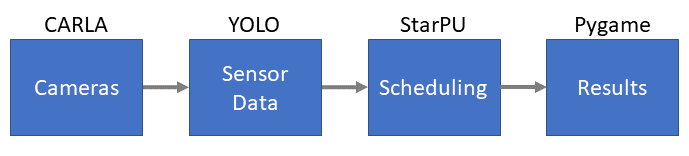
\includegraphics[width=0.9\linewidth]{Figure1d.png}
\caption{System Overview}
\label{esquema}
\end{figure}
%[width=\linewidth]

%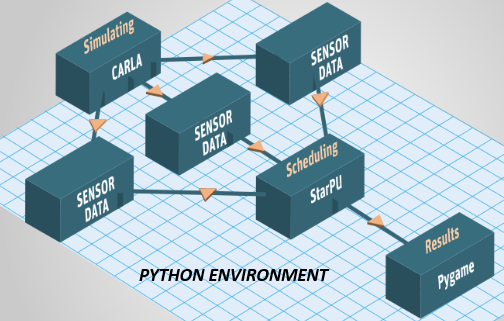
\includegraphics[width=\linewidth, height=0.1\textheight]{Figure3b.png}

One of the main contributions of this paper is the integration of CARLA for realistic simulations and StarPU for efficient resource management to improve ADV task scheduling. To the best of our knowledge, this is the first study to explore that. The second contribution is the exploration of different strategies for task scheduling in a heterogeneous system comprising GPU/CPU processing units to improve task execution times and overall system performance. For this, we designed an ADV virtual model up to the sensor processing management by the CARLA simulator. The remainder of this paper is organized as follows: Section II presents Related Work, Section III is the Experimental Setup, Section IV shows the Results and Discussion, and finally, Section V describes our conclusions.


\section{Related Work}

\subsection{Task Scheduling for Autonomous Vehicles}

%Efficient task management is essential for handling intense computational tasks that ADV must process in real-time. It ensures safety, minimizes task miss rates, and optimizes computing resource utilization. It enables ADV to make decisions without losing its optimal performance. However, finding the optimal strategy to save energy consumption and minimize execution time remains challenging for many researchers.

In the work by Balasekaran et al. \cite{Balasekaran2021}, the authors propose an intelligent task scheduling mechanism for autonomous vehicles that uses deep learning algorithms. Their method focuses on reducing execution time and improving resource utilization using a single-layer feedforward neural network (SLFN) for task distribution. Tasks are scheduled using an Earliest Hyper Period First (EHF) scheduler, which helps minimize the task miss rate and energy consumption. This approach was validated on multicore System-on-Chip (SoC) platforms.

Dai et al. \cite{Dai2019} present a scheduling algorithm for ADV tasks using mobile edge computing (MEC). The system offloads computationally intensive tasks to edge servers, considering that the ADV onboard computational systems are limited in battery life and computing capabilities. Their strategy uses an improved Earliest Deadline First (EDF) algorithm to manage task scheduling with task migration from servers. For this approach to work, the authors rely on the speed of the 5g wireless networks to improve data exchange between vehicles and servers.

Also dealing with edge servers and vehicular networks, Qi et al. \cite{qi2020} focus on parallel task scheduling, combining edge computing with deep reinforcement learning to improve task allocation. They developed a distributed multilevel task scheduling (MDTS) algorithm to assign tasks to edge nodes, prioritizing load balance and total execution cost. This method focuses on learning from the environment to dynamically allocate tasks across various processing nodes, including on-board processors and MEC servers.

Amarnath et al. \cite{amarnath2021} present a heterogeneity-aware task scheduling algorithm (HetSched) designed for SoCs in ADV. Dynamically prioritizes tasks based on the variation in execution time between different processing elements of the SoC. It prioritizes safe-critical tasks and trims the ones that are not essential and could not meet the requirements to improve the ADV mission time. It uses the STOMP scheduler platform \cite{vega2020}  to evaluate its designed algorithm.

Furthermore, Xu et al. \cite{Xu2022} propose the Age of Information (AoI)-centric task scheduling approach that aims to ensure that tasks use the most recent sensor data, which is critical for correct detection, planning, and action taking by ADV. The schedule uses a reinforcement learning solution by integrating its scheduler with a Double deep Q network (DQN) to solve hard combinatorial problems. %This approach was tested and validated in the Appolo driving system \cite{ApolloSelfDriving2024}.

Existing approaches frequently face challenges such as rigid, platform-specific implementations that lack flexibility for heterogeneous systems. Additionally, theoretical scheduling models are often validated only in constrained environments, and high overhead from edge computing or complex reinforcement learning models makes them unsuitable for real-time applications.


%This paper differs from previous ones, as it does not look to validate a specific platform or strategy in a theoretical fashion with a limited focus on practical integration. 

In contrast, this work aims to build a scheme that could test any developed task scheduling plan by simply porting it to Python language in a common working environment. It will allow users to apply well-established or novel-designed scheduling strategies or develop their own, providing a practical, real-world platform to manage heterogeneous task scheduling. By exploring the possibilities of integrating simulation software with a runtime system for task scheduling, it aims to offer dynamic task management and resource allocation strategies in a realistic driving environment to achieve results as close as possible to those achieved with ADV prototypes. 



\subsection{Simulation/System Integration for Autonomous Vehicles}

%Simulators have become indispensable in the development of ADV, especially in terms of safety and cost, and they can validate algorithms and vehicle behavior under a range of conditions. It is unnecessary to spend many hours on the streets and roads facing hazards and consuming fuel. Simulators have considerably evolved and face challenges like sensor fidelity and vehicle dynamics. It is rapidly evolving, with new software being deployed regularly.

Rosique et al. \cite{Rosique2019} provide a comprehensive overview of the available simulators. They classified simulators into four main types: model-based development simulators, robotics simulators, game engine-based simulators, and AV-specific simulators. It was highlighted that perception subsystems, such as LIDAR, cameras, and RADAR, are essential to create high-fidelity simulation conditions. However, they identified shortcomings in computational efficiency and the processing of large-scale simulations.

Five years later, Li et al. \cite{Li2024} provided an updated and more detailed exploration of the evolution of simulators. It offers new classification categories for simulators: traffic flow, sensory data, driving policy, vehicle dynamics, and comprehensive simulators. This last category mainly includes all-in-one solutions that comprise all previous categories, yet it is mostly proprietary software. It is important to note the large number of new software deployed after the work of \cite{Rosique2019} in 2019. In \cite{Li2024}, advances in simulation technology, particularly in high-fidelity environments and the inclusion of various driving conditions, were discussed to make simulators more relevant for testing complex driving policies and end-to-end systems. However, limitations in computational performance and experimental reliability were pointed out, particularly when scaling simulations for real-world ADV applications. It also advocates that the key feature to get the simulation as close to the real world as possible is integrating real-time frameworks used in ADV prototypes such as ROS2 \cite{ros} and Autoware \cite{kato2018}.

%Both previous references considered the CARLA simulator the most complete open-source software and the only one in this category that is still being updated. CARLA offers a variety of predefined integrations to supply what the simulator environment lacks, the so-called CARLA ecosystem. Follow the most notable ones. 

%Integration with AWS \cite{kewate2022} to train reinforcement learning algorithms.
Connection to CARSIM \cite{carsim} or Chrono \cite{chrono} where vehicle controls and dynamics are handed to an external simulator and returned to CARLA only the state and location of the vehicle. Integration with Robot Operating System (ROS) \cite{ros} versions 1 and 2 takes advantage of CARLA high-definition maps to visualize the environment while keeping control of all other aspects such as spawning actors, sensors data processing, and vehicle control. 

Furthermore, it does a co-simulation with Sumo \cite{sumo} and PTV-Vissim \cite{ptv_vissim}, where the simulation is synchronized, and the user can explore and choose the capabilities of each simulator. However, there is no integration with any tools that would focus solely on improving execution performance or managing and distributing the tasks to be executed.


\section{Experimental Setup}
In this section, we describe the whole setup, starting from the vehicle deployment and the attachment of sensors using the CARLA simulator environment. The data of these sensors are processed to obtain meaningful information. This is done by organizing them into tasks composed of sensor and processing algorithms and sending them to the StarPU task management to apply scheduling techniques. The simulation runs on a machine with Ubuntu 20.04 as an operating system equipped with an i5-10400 processor with six cores, a Geforce RTX 3060 GPU, and 32GB of DDR4 RAM.

\subsection{CARLA simulator}
CARLA (Car Learning to Act) is an open-source simulation platform designed to facilitate the development, testing, and validation of autonomous driving systems \cite{Dosovitskiy2017}. It provides an urban environment where researchers can simulate complex driving conditions, including changes in weather, pedestrian movements, and vehicle behaviors. Built on Unreal Engine 4, CARLA offers high-fidelity 3D environments, making it suitable for academic research and industry applications. %\cite{CARLA}

CARLA's sensor suite, which includes cameras, LIDAR, radar, and GPS, permits developers to simulate a wide range of real-world conditions. This supports the testing of perception, localization, and control algorithms. Moreover, CARLA offers flexible API support, enabling integration with Python and C++ for logical interaction with autonomous driving stacks. The platform is also highly customizable, allowing users to modify the environment, sensor settings, and traffic scenarios, creating a rich testing ground for autonomous systems.

%The platform also supports multi-agent simulation, where multiple autonomous agents, such as vehicles and pedestrians, interact in complex traffic environments. This multi-agent setup enables testing autonomous driving algorithms in scenarios involving diverse traffic behaviors. The software also integrates HD maps and OpenDrive standards, facilitating realistic vehicle dynamics and road infrastructure simulations. 

\subsection{StarPU Runtime System}

StarPU is a runtime system designed to schedule and manage tasks on heterogeneous computing platforms efficiently. Its main purpose is to enable the smooth execution of heterogeneous applications on hardware with varying architectures, such as multicore CPUs, GPUs, and other accelerators \cite{augonnet2009}. By abstracting the complexities of heterogeneous hardware, StarPU allows developers to focus on optimizing their algorithms without needing to manage the complexity of hardware-specific execution manually.

One of the key features of StarPU is its dynamic scheduling ability, where the system selects the most appropriate hardware resource, such as CPU, GPU, FPGA, and DSP, to execute each task based on the current system load and task requirements. This dynamic resource allocation helps improve overall system performance and task execution efficiency. StarPU achieves this through various scheduling policies, such as work-stealing, priority-based scheduling, and data locality optimization, which ensure that the workload is balanced across available resources while minimizing communication overhead \cite{StarPU}.

%Additionally, StarPU provides a performance feedback mechanism in which the runtime system monitors and collects performance metrics during execution. This feedback allows the system to adapt its scheduling strategies dynamically, optimizing task placement based on runtime conditions. It also supports task-based parallelism, where computational tasks are expressed as a directed acyclic graph (DAG). Furthermore, StarPU has a memory management system that automatically handles data transfers between different memory spaces (e.g., CPU and GPU memory), reducing the burden on developers to manage low-level memory operations.


\subsection{Simulation Environment}\label{AA}
%In the CARLA simulator space, spawning is deploying something into the simulated world: sensors, infrastructure, pedestrians, or vehicles, which the API calls actors. Hence, two simulation setups with two different vehicles were spawned in the API as actors in the CARLA environment. Setup 1 was a randomly generated vehicle with eight attached RBG cameras that processed images in real-time. The cameras covered 360 degrees of field of view, with an angular difference from each other of 45 degrees. Setup 2 was a Tesla Cybertruck with more sensors than the previous setup composed of 6 cameras pointing to the front, left, right, rear, front-left, and front-right, a LIDAR, a Radar, an IMU, and a GNSS. Figure \ref{setups} shows a vehicle setup used in the simulations.

In the CARLA simulator space, spawning is deploying something into the simulated world: sensors, infrastructure, pedestrians, or vehicles, which the API calls actors. Figure \ref{setups} shows a vehicle setup used in the simulations based on a Tesla Cybertruck composed of eight cameras that dynamically cover a field of view of 360 degrees.

\begin{figure}[htbp]
\centering
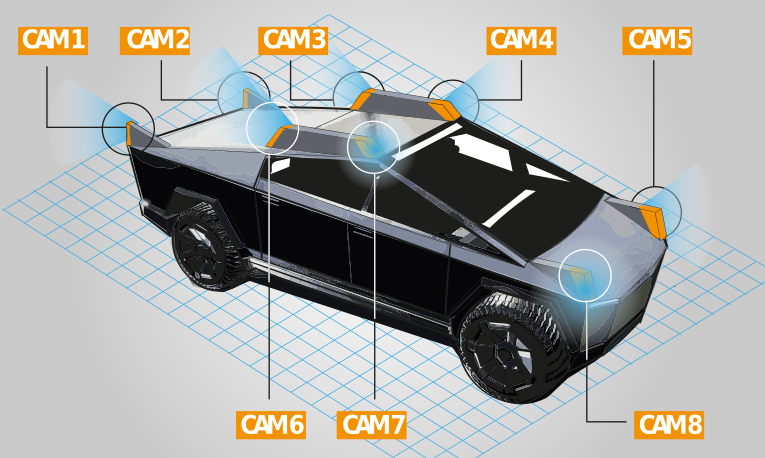
\includegraphics[width=\linewidth, height=0.17\textheight]{Figure1.png}
\caption{Vehicle Setup}
\label{setups}
\end{figure}
%[width=\linewidth]


The Carla server was loaded with the Town10 map, a downtown urban suburb with residential buildings on its outskirts and skyscrapers in its central area. In addition, pedestrians and other vehicles were spawned on the map, and their movement was set to auto-mode to best simulate a city environment. In addition, the main vehicle was running in auto mode to continue moving around the city to record data using the sensors.

To visualize sensor information and see vehicle location, a PyGame \cite{Kelly2016} was deployed, generating a window subdivided into small sub-windows for each camera spawned in the vehicle to visualize processed data from all sensors. Figure \ref{pygame} shows how the data were visualized.

\begin{figure}[htbp]

\includegraphics[width=\linewidth, height=0.17\textheight]{Figure2.png}
\caption{PyGame Visualization Window}
\label{pygame}
\end{figure}

\subsection{Sensor Data Processing}

%Sensor data are processed in the simulations to detect objects and the vehicle's surroundings. Algorithms must be applied specifically to each type of data.

%\cite{Redmon2016}

In the RGB camera image, the Yolo algorithm (You Only Look Once) was utilized to detect objects in the provided camera feed. This algorithm was created in 2015 and quickly gained popularity due to its accuracy, high speed, and lightweight. Using a convolutional neural network (CNN) to scan the entire picture simultaneously, it can process images at 45 frames per second and segment them into small boxes with meaningful identification. In this simulation, we used version 5 of the algorithm with a pre-trained database maintained by Ultralytics \cite{ultralytics2024}, which now hosts and maintains the algorithm. This version is simple and robust, compatible with Python 3.7 to 3.9, which is in the range of compatibility with the CARLA simulator. Yolo received 640x360 pixels images at 20 frames per second.

% The following algorithms were used only in simulation setup two as it has other sensors.

%\cite{Brilli2018}

%Carla simulator enables the spawning of a rotating LIDAR raycast sensor that generates a cloud of points that maps the scene. For dealing with LIDAR point cloud data to detect objects, a DBSCAN (Density-Based Spatial Clustering of Applications with Noise) algorithm is applied \cite{Ester2016}. It does point clustering based on the density of the sensor data. The points cloud is clustered by grouping nearby points while filtering out noise or isolated points.

%To obtain vehicle location within the simulation map, a sensor fusion technique of the GNSS (Global Navigation Satellite System) and IMU (Inertial Measurement Unit) was used. The reason for combining these sensors is because they are limited to being used alone. On the one hand, GNSS is not ideal for real-time applications and can be noisy and subject to signal loss; on the other hand, IMU tends to drift over time. The method explained in \cite{falletti2011} was applied to get an accurate real-time position. It fuses both sensor signals using the Kalman Filter. The IMU high-rate motion estimation is adjusted by the GNSS, thus reducing the drift and returning a more accurate real-time ADV position.

%\cite{li2015}

%The radar sensor is used to detect objects that are near the vehicle in the simulation. We use a custom algorithm to separate the detected objects into three categories: vehicles, pedestrians, and infrastructure. That is done by the speed of the object detected by the radar. If its speed is greater than 2.0 m/s, it is classified as a vehicle; if it is less than this, it is classified as a pedestrian; and if it is a static object, it is classified as infrastructure. The processed data are visualized based on their depth, altitude, and azimuth. Different colors are used to distinguish the detected objects in the visualization Pygame display.

%Finally, all objects detected by the previous sensors were fused to generate a cost map using an occupancy grid map. % \cite{meng2022}
%This works by dividing the environment into cells where each has a probability of being occupied. Furthermore, a Bayesian updating method \cite{Yin2021} was applied to refine the occupancy prediction based on sensor data. The final result is a generated 2D grip map occupied by the detected objects from LIDAR, Radar, and Cameras. 

The sole objective of processing sensor data with complex algorithm is to generate enough workload to get meaningful results and investigate the advantages of applying the task scheduling techniques to an ADV processing pipeline in its heterogeneous system. Furthermore, the cameras were considered enough workload for the ADV's perception system. Hence, it did not include algorithms related to the planning and control parts of the ADV Architecture\cite{Silva2024}.

\subsection{StarPU Integration}
StarPU was integrated into the CARLA simulation using Python, a common language that allows communication between the two libraries through their APIs. This allowed us to manage and schedule the computational workload from the cameras and the Yolo algorithm. %, as explained in the previous section.

The first step is to define the tasks that StarPU will manage. Each task was defined as composed of raw data and an algorithm to process these data. For that to happen, the sensor data and its processing algorithm must be defined within a Python function. This function becomes a task. This task can be submitted using a decorator for the function or explicitly submitting it with a StarPU submit task command. Despite that, other workloads from the simulation, such as vehicle control and Pygame visualization windows, were not sent to StarPU management.
   %Following the rules mentioned, we created two vehicle setups composed of task functions, where one task for each camera (8 in setup 1 and 6 in setup 2), five tasks for the LIDAR, Radar, IMU, GNSS, a localization task, and one costmap task with the sensor detection fusion in it. 

%An important observation is that the action to spawn and prepare the vehicle and the environment was not considered in this processing setup. The reason is that in the real prototype, these are its infrastructure, so to make the simulation as close as possible to the real vehicle, any processing not done in the real machine was not handled by StarPU.

StarPU can dynamically schedule tasks and manage their distribution through the GPU and CPU processing nodes, following a scheduling strategy defined inside the code or as an option at the time of executing the script. It offers a range of strategies that can be quickly changed every time the script is executed using the option STARPU\_SCHED. The Python time library was used to measure the execution time for each task and the iteration time of the full simulation.
%,  this last one including the workload managed and not managed by StarPU.



\section{Results and Discussion}

\subsection{StarPU integration into CARLA simulation}
The integration of StarPU with the CARLA simulator demonstrated an interesting way to manage the computational workload in ADV. This paper focused on managing sensor processing for object detection tasks, but this approach could be extended to the entire ADV processing pipeline, including navigation and vehicle control. 

Using StarPU, it was possible to submit vehicle processing tasks as Python functions simply by using the function \textit{starpu.task.submit}. It is important to note the relevance of the library \textit{asyncio} for the proper execution of StarPU as it gives the necessary flexibility of asynchronous execution, which is required when programming in a task-oriented manner. In addition, it allowed task submission parallelism without relying on multiple threads since, in Python, they are limited by the Global Interpreter Lock (GIL), preventing the language from having real parallelism.

As seen in Figure \ref{pygame}, during the simulation, a real-time display of the task processing times individually and the total iteration time was created using PyGame. This feedback allowed for the verification of task scheduling performances during vehicle navigation on the map in autopilot. Hence, it was possible to identify performance bottlenecks and the impact of different scheduling strategies.

\subsection{Application of Scheduling Strategies}

We evaluated the impact of different scheduling strategies on the performance of the ADV sensor processing pipeline using several scheduling algorithms provided by StarPU. The recorded times are presented in this section. The scheduling strategies used in this paper are as follows:

\begin{itemize}
    \item \textbf{WS}: Work-Stealing
    \item \textbf{LWS}: Local Work-Stealing
    \item \textbf{PRIO}: Priority-based
    \item \textbf{RANDOM}: Random task allocation
    \item \textbf{HETEROPRIO}: Heterogeneous Priority
    \item \textbf{EAGER}: Eager scheduling
    \item \textbf{DMDA}: Deque Model Data Aware
    \item \textbf{PHEFT}: Parallel Heterogeneous Earliest Finish Time
    \item \textbf{PEager}: Parallel Eager scheduling
    \item \textbf{OSOnly}: The operating system handles tasks %No StarPU scheduling strategy;
\end{itemize}

% After checking, revert to regular color:
The scheduling strategies helped us identify performance differences in the ADV sensor processing pipeline.
 Every scheduling strategy was running for 2000 full code iterations. The following results summarize the performance of various scheduling strategies in terms of Average Iteration Time, Average Task Time, CPU Usage, and GPU Usage.

It is important to note that, although StarPU was responsible for managing the workload of the cameras and their processing algorithms, the performance metrics were measured across the entire simulation loop.

%, including iteration time and the device usage of both the CPU and GPU.
%power consumption

\subsubsection{Iteration Time}



\begin{table}[h]
\centering
\caption{Performance for Different Scheduling Strategies}
\label{table}
\begin{tabularx}{\columnwidth}{l *{4}{>{\centering\arraybackslash}X}}
\toprule
\textbf{Scheduling Strategy} & \textbf{Avg Iteration Time (sec)} & \textbf{Avg Task Time (sec)} & \textbf{Avg CPU Usage (\%)} & \textbf{Avg GPU Usage (\%)} \\
\midrule
WS           & 0.0777 & 0.0266 & 29.8274 & 80.0350 \\
LWS          & 0.0697 & 0.0478 & 35.7746 & 84.0919 \\
PRIO         & 0.0795 & 0.0195 & 27.3814 & 78.1834 \\
Random       & 0.0716 & 0.0374 & 33.4894 & 84.3138 \\
HeteroPrio   & 0.0709 & 0.0466 & 35.1347 & 85.2222 \\
Eager        & 0.0774 & 0.0196 & 28.1366 & 79.0994 \\
DMDA         & 0.0690 & 0.0475 & 35.5200 & 85.2729 \\
PHEFT        & 0.0785 & 0.0227 & 29.2147 & 79.3250 \\
PEager       & 0.0781 & 0.0188 & 27.8244 & 78.5460 \\
OSOnly   & 0.0804 & 0.0154 & 26.6940 & 77.5979 \\
\bottomrule
\end{tabularx}
\end{table}



%\begin{table}[h]
%\centering
%\caption{Performance for Different Scheduling Strategies}
%\label{table}
%\begin{tabularx}{\columnwidth}{l *{6}{>{\centering\arraybackslash}X}}
%\toprule
%\textbf{Scheduling} \\ \textbf{Strategy} & \textbf{Avg Iteration Time (sec)} & \textbf{Std Dev Iteration Time (sec)} & \textbf{Avg Task Time (sec)} & \textbf{Std Dev Task Time (sec)} & %\textbf{Avg CPU Usage (\%)} & \textbf{Avg GPU %Usage (\%)} \\
%\midrule
%WS           & 0.0777 & 0.0087 & 0.0266 & 0.0165 %& 29.8274 & 80.0350 \\
%LWS          & 0.0697 & 0.0080 & 0.0478 & 0.0148 %& 35.7746 & 84.0919 \\
%PRIO         & 0.0795 & 0.0078 & 0.0195 & 0.0148 %& 27.3814 & 78.1834 \\
%Random       & 0.0716 & 0.0092 & 0.0374 & 0.0147 %& 33.4894 & 84.3138 \\
%HeteroPrio   & 0.0709 & 0.0073 & 0.0466 & 0.0135 %& 35.1347 & 85.2222 \\
%Eager        & 0.0774 & 0.0059 & 0.0196 & 0.0037 %& 28.1366 & 79.0994 \\
%DMDA         & 0.0690 & 0.0063 & 0.0475 & 0.0091 %& 35.5200 & 85.2729 \\
%PHEFT        & 0.0785 & 0.0092 & 0.0227 & 0.0154 %& 29.2147 & 79.3250 \\
%PEager       & 0.0781 & 0.0033 & 0.0188 & 0.0017 %& 27.8244 & 78.5460 \\
%OSOnly       & 0.0804 & 0.0045 & 0.0154 & 0.0148 %& 26.6940 & 77.5979 \\
%\bottomrule
%\end{tabularx}
%\end{table}


The average iteration time is a critical metric of the ADV that represents the overall speed of the simulation loop. A lower iteration time indicates a more efficient scheduling strategy to process simulation steps faster, which is essential for real-time autonomous vehicle applications. The items created in CARLA, such as vehicles, pedestrians, and cameras, are not included in the simulation loop, nor is the visualization in the Pygame window, which is also outside of the StarPU processing tasks. 

%As illustrated in

Table \ref{table} shows that the DMDA scheduling strategy achieved the lowest average iteration time, 0.06899 seconds, outperforming all other strategies. This suggests that DMDA effectively balances the workload between CPU and GPU resources, minimizing idle times and overhead as a data-driven scheduling strategy. It also requests that the task performance model be configured as an option in the StarPU task submit function to work correctly in the StarPU environment. Following DMDA, the LWS and HeteroPrio strategies also shows competitive average iteration times of 0.06966 seconds and 0.07092 seconds. In contrast, the OSOnly script exhibits the highest average iteration time of 0.08038 seconds. %\textcolor{red}{indicating that integrating with StarPU and exploring heterogeneous scheduling can improve simulation performance}. 


Further analyses can be performed by verifying the evolution of iteration time over iterations, as seen in Figure \ref{itergraph}. It confirms the good results of DMDA, HeteroPrio, and LWS while maintaining a low iteration with feel spikes indicating better balance and resource utilization. These strategies, in many points, can reduce the iteration time up to 40\% of the average. PRIO and PEager also show promising results but with more oscillations, which affects its overall performance. OSOnly tends to have the most stable but higher iteration time, as seen in Table \ref{table}, which is expected due to the nonexistence of StarPU scheduling strategy since the operating system handles tasks. Random shows good results but more frequent and unpredictable spikes, which indicates it's difficult to consistently allocate tasks over time.

%its simplicity and scheduling without optimizations. 

\begin{figure}[htbp]

\includegraphics[width=\linewidth, height=0.185\textheight]{Figure5.png}
\caption{Iteration Times over Iterations}
\label{itergraph}
\end{figure}

\begin{figure}[htbp]
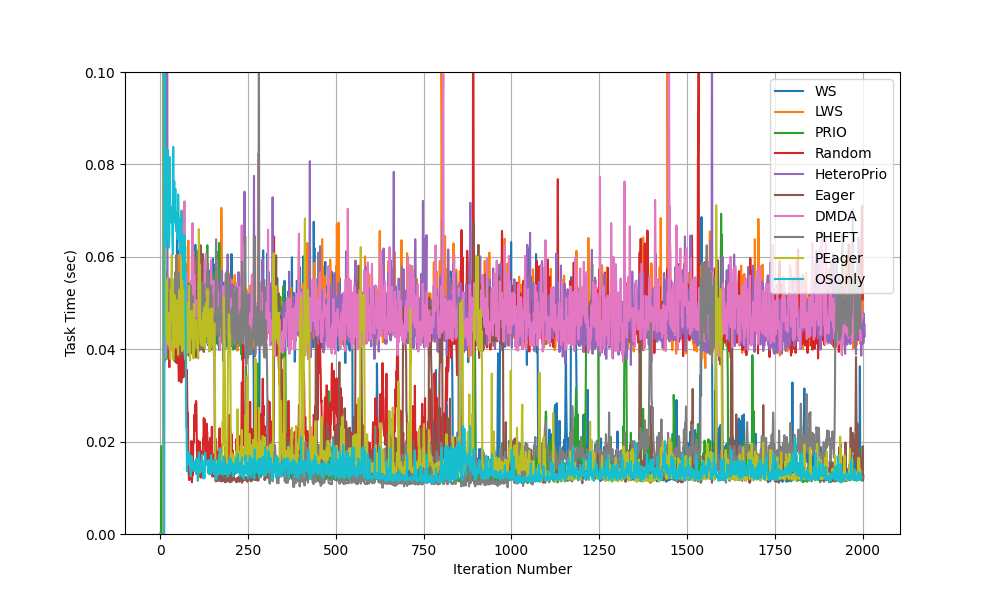
\includegraphics[width=\linewidth, height=0.185\textheight]{Figure6.png}
\caption{Task Times over Iterations}
\label{tasktime}
\end{figure}


\subsubsection{Task Time}
The average task time measures the time to execute individual tasks within the simulation. Again, the only tasks submitted are related to the cameras' image processing. The average recordings could be verified in Table \ref{table} and also in Figure \ref{tasktime}. It could be seen that the scheduler needed some time to settle up and stabilize its execution of above 100 iterations. In addition, the constant oscillation in the average task time could be due to the constant variability of the cameras' input data, as the collected data varies significantly depending on the number of objects detected.

It could also be verified that the scheduling policies are separated into two groups. WS, PRIO, Eager PHEFT, and OSOnly have small task times compared to LWS, Heteroprio, and DMDA. However, this did not necessarily translate into overall performance. For example, the OSOnly strategy recorded the lowest average task time of 0.01543 seconds. However, its longer iteration time proved inefficiencies at the simulation loop level, possibly because of the lack of optimization of the utilization of computing resources. Similarly, the PEager and PRIO strategies also showed low average task times of 0.01882 seconds and 0.01948 seconds but did not achieve the highest performance.

StarPU is a runtime system that introduces overhead and its scheduling performance improves with increasing workloads. The better task time performance of OSOnly can be explained by the absence of this overhead. In this paper, we conducted a controlled experiment to validate the CARLA/StarPU integration under scheduling evaluation. As discussed in future work, larger workloads will be evaluated to propose a new scheduling strategy.

%This could be attributed to the absence of scheduling overhead associated with StarPU, which allows tasks to be executed without additional latency.

%respectively, but did not achieve optimal performance.

\subsubsection{Resource Utilization}

Efficient utilization of CPU and GPU resources is crucial for optimizing performance in a heterogeneous computing system. Higher resource usage typically leads to better performance, provided the resources are appropriately applied. As can be seen in Figure \ref{usage}, the DMDA strategy not only achieved the lowest iteration time but also had the highest GPU usage at 85.25 \% and the second highest CPU usage at 35.52 \%. This utilization indicates that DMDA effectively explores CPU and GPU resources, leading to improved performance. The HeteroPrio and LWS strategies perform close to DMDA performance, showing that these are the options for heavy GPU workloads.

%, as seen in the previous sections

\begin{figure}[t] % Use [t] to position the figure at the top of the column
\centering
\begin{adjustbox}{width=\columnwidth}
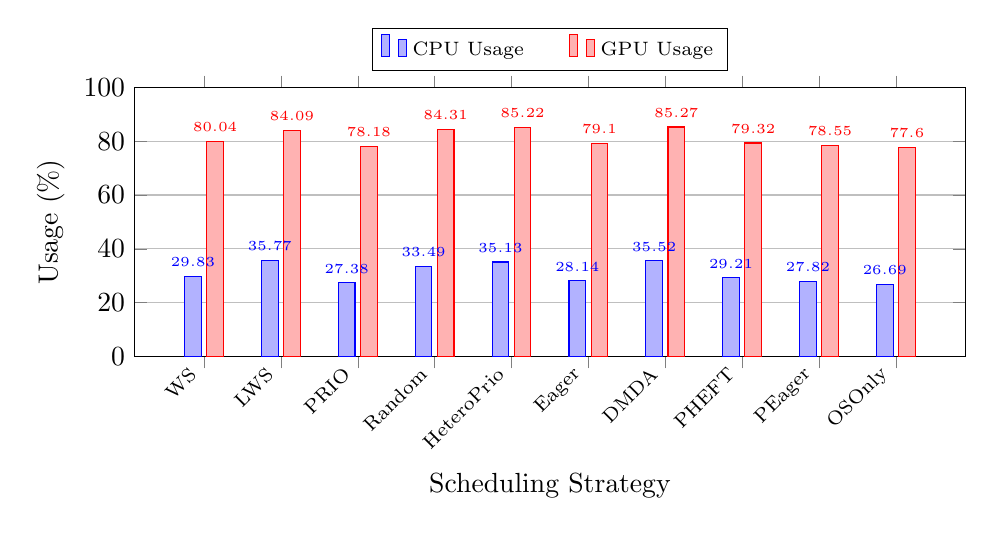
\begin{tikzpicture}
\pgfplotstableread{
Strategy        CPU     GPU
WS              29.83   80.04
LWS             35.77   84.09
PRIO            27.38   78.18
Random          33.49   84.31
HeteroPrio      35.13   85.22
Eager           28.14   79.10
DMDA            35.52   85.27
PHEFT           29.21   79.32
PEager          27.82   78.55
OSOnly      26.69   77.60
}\datatable

\begin{axis}[
    ybar,
    bar width=6pt,
    width=\columnwidth,
    height=5cm, % Increased height from 6cm to 7cm
    legend style={
        at={(0.5,1.06)}, % Moved legend above the plot
        anchor=south, % Anchored the legend to the bottom center
        legend columns=2,
        font=\scriptsize,
        /tikz/every even column/.append style={column sep=0.5cm} % Added space between legend columns
    },
    symbolic x coords={WS,LWS,PRIO,Random,HeteroPrio,Eager,DMDA,PHEFT,PEager,OSOnly},
    xtick=data,
    x tick label style={rotate=45, anchor=east, font=\scriptsize, yshift=0.5ex}, % Adjusted yshift
    ylabel={Usage (\%)},
    xlabel={Scheduling Strategy},
    ymin=0, ymax=100,
    ymajorgrids=true,
    nodes near coords,
    nodes near coords style={font=\tiny},
    nodes near coords align={vertical},
    ]

\addplot+[blue,fill=blue!30] table[x=Strategy,y=CPU]{\datatable};
\addplot+[red,fill=red!30] table[x=Strategy,y=GPU]{\datatable};

\legend{CPU Usage, GPU Usage}

\end{axis}
\end{tikzpicture}
\end{adjustbox}
\caption{CPU and GPU Usage for Each Scheduling Strategy}
\label{usage}
\end{figure}


On the other hand, the OSOnly strategy had the lowest CPU (26.69 \%) and GPU (77.60 \%) usages, aligning with its higher iteration time. This suggests that OSOnly does not fully explore the available hardware resources, leading to less efficient simulation performance.


\section{Conclusions}

This paper successfully integrated the CARLA simulator and the StarPU runtime system, exploring various scheduling strategies for autonomous vehicles. This integration demonstrated the potential for optimizing perception tasks in a heterogeneous computing environment applied to ADV. However, the study is limited to simulated sensor data that could have discrepancies compared to real world results. Despite the limitations, results showed that the dynamic allocation of tasks across CPUs/GPUs significantly improved task execution efficiency. The DMDA scheduling strategy achieves the best overall performance despite the higher processing time per task.

% This approach enhances the flexibility of task management strategies development and paves the way to simulate and optimize the full pipeline of an ADV.

Future work focuses on increasing the number of sensors and data processing algorithms, covering the other parts of the ADV pipeline, e.g., localization, decision-making, and control. Additionally, advances in high-performance computing hardware, such as specialized AI accelerators, are expected to open new possibilities for improving task execution efficiency including the integration of machine learning-based adaptive scheduling algorithms.


%We also intend to develop and evaluate a machine learning-based scheduling strategy.
%
%
% handled in a simulated environment
%\textcolor{red}{and to use a more specific measurement technique to pinpoint direct StarPU impact on performance}.





%\section*{Acknowledgment}

%The preferred spelling of the word ``acknowledgment'' in America is without 
%an ``e'' after the ``g''. Avoid the stilted expression ``one of us (R. B. 
%G.) thanks $\ldots$''. Instead, try ``R. B. G. thanks$\ldots$''. Put sponsor 
%acknowledgments in the unnumbered footnote on the first page.


\bibliographystyle{IEEEtran}
\bibliography{references.bib}



%\vspace{12pt}
%\color{red}
%IEEE conference templates contain guidance text for composing and formatting conference papers. Please ensure that all template text is removed from your conference paper prior to submission to the conference. Failure to remove the template text from your paper may result in your paper not being published.

\end{document}
